\documentclass[a4paper,10pt,oneside]{report}%pridat twoside, do [] pre obojstrannu tlac
\pagestyle{headings}
\usepackage[top=2.5cm, bottom=2.5cm, left=3.5cm, right=2cm]{geometry} %odporucane okraje
\linespread{1.50}

%% Generally used
\usepackage{ebproof}
\usepackage{amsthm}
\usepackage{amsmath}
\usepackage{amssymb, upgreek}
\usepackage{mathtools}
\usepackage{color}
\usepackage{pdfpages}
\usepackage[slovak]{babel}
\usepackage[T1]{fontenc}
%% Generally used

% USE PACKAGE BABEL SLOVAK

\renewcommand{\thesection}{\arabic{section}}

%% Lean specific
\usepackage[utf8x]{inputenc}
\definecolor{keywordcolor}{rgb}{0.7, 0.1, 0.1}   % red
\definecolor{commentcolor}{rgb}{0.4, 0.4, 0.4}   % grey
\definecolor{symbolcolor}{rgb}{0.0, 0.1, 0.6}    % blue
\definecolor{sortcolor}{rgb}{0.1, 0.5, 0.1}      % green
\definecolor{errorcolor}{rgb}{1, 0, 0}           % bright red
\definecolor{stringcolor}{rgb}{0.5, 0.3, 0.2}    % brown
\usepackage{pict2e,picture}

\usepackage{listings}
\def\lstlanguagefiles{lstlean.tex}
\lstset{language=lean}
%% Lean specific

%% Covering

\newcommand{\coveringA}{%
  \mathrel{-\mkern-4mu}<%
}
\newcommand{\coveringB}{\mathrel{\text{$\vcenter{\hbox{\pictcoveringB}}$}}}

\newcommand{\pictcoveringB}{%
  \begin{picture}(1em,.5em)
  \roundcap
  \put(0,.25em){\line(1,0){.6em}}
  \put(.6em,.25em){\line(3,1){.4em}}
  \put(.6em,.25em){\line(3,-1){.4em}}
  \end{picture}%
}
%% Covering

%% Powerset
\newcommand{\powerset}{\raisebox{.15\baselineskip}{\Large\ensuremath{\wp}}}
%% Powerset
\newcommand{\nothing}{\varnothing}

\newtheorem{theorem}{Veta}[chapter]
\newtheorem{definition}{Definícia}[chapter]

\author{Mat\'u\v{s} Behun}
\title{Dokazovanie viet v systéme Lean}

\begin{document}

%\setlength{\belowdisplayskip}{7pt} \setlength{\belowdisplayshortskip}{5pt}
%\setlength{\abovedisplayskip}{7pt} \setlength{\abovedisplayshortskip}{5pt}


%\thispagestyle{empty}
%{
    %\topmargin=0pt
    %\centerline {\large \bf{Slovenská technická univerzia v Bratislave}}
    %\vskip 0.2cm
    %\centerline{\large \bf{Stavebná fakulta}}
    %\vskip 0.2cm
    %Evidenčné číslo: SvF-5343-54946 
    %\vskip 5.0cm
    %\centerline{\Large \bf{Dokazovanie viet v systéme Lean}}
    %\vskip 0.2cm
    %\vskip 0.5cm
    %\centerline{\large \bf{Diplomová práca}}
    %\vskip 7cm          %\vskip 2cm             %zmena kvoli zobrazovaniu dnesneho datumu
    %\normalsize
    %\begin{tabular}[l]{p{0.27\textwidth}p{0.73\textwidth}}
        %Študíjny program: & matematicko počítačové modelovanie  \\
        %Odbor: & matematika  \\
        %Department: & Katedra matematiky a deskriptívnej geometrie\\
        %Vedúci práce: & doc. Mgr. Gejza Jenča, PhD. \\
    %\end{tabular}
    %\vskip 3cm
    %\centerline{\large \bf{Bratislava 2021}}
    %\vskip 0.2cm
    %\centerline{\large \bf{Mat\'u\v{s} Behun}}
%}

%\newpage

%% Odkomentovat
%%% 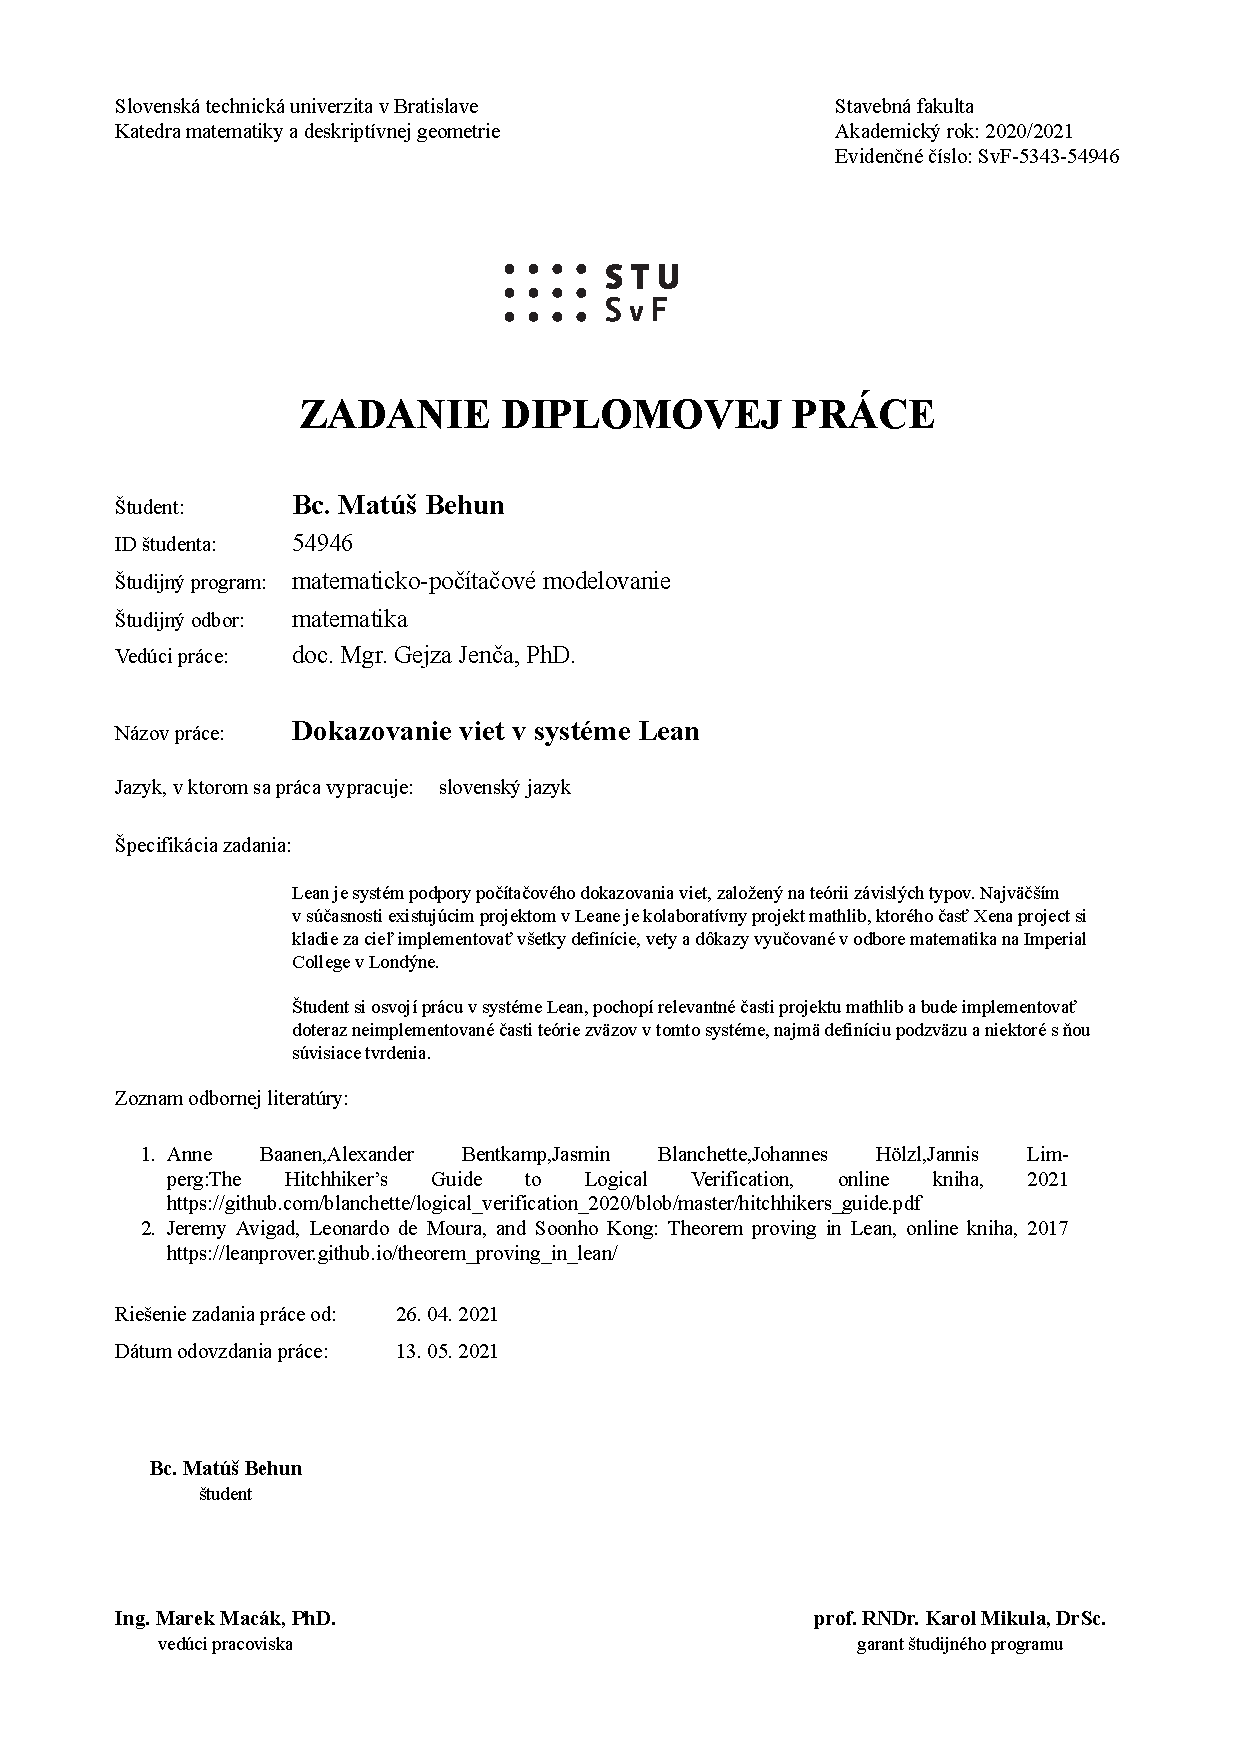
\includepdf[pages={1}]{zadanieDiplomovka.pdf}

%\newpage

\tableofcontents

\newpage

\chapter{Úvod}
    Dokazovací asistenti obsahujú interaktívne prostredie ktoré na základe vstupu
používateľa tvoria formálne dôkazy.
    Táto diplomová práca sa zaoberá dokazovacíom asistentom Lean ktorý je
založený na teórii závistlostných typoch.
    V úvode práce uvádzame teoreticky nevyhnutú časť intuicionistickej logiky
a jednoduchej teórie typov aby sme ukázali prepojenie medzi logikou a výpočtovými
modelmi ktoré je známe ako Curry-Howardova izomorfizmus.

    Druhá kapitola opisuje prostredie Lean-u, jeho základnú syntax a prácu s 
typmi ktoré sú jeho základným prvkom.
    Poskytujeme pohľad na dva spôsoby dokazovania. Dopredným spôsobom ktoré je priamym
poskytnutím $\lambda$-výrazu, a spätným v taktickom móde ktoré naplno využíva interaktívne prostredie.
    Kapitolu uzatvárame opisom syntaxe využívanej na budovanie štruktúr používanej
pri tvorbe tých matematických a ich hierarchie.

    V poslednej kapitole rozoberáme našu implementáciu vety o izomorfizme modulárnych
zväzov.
    Opisujeme základné definície a štruktúry týkajúce sa teórie čiastočného usporiadania
implementovaných v rámci komunitného projektu mathlib.
    Na záver podrobne opisujeme náš príspevok štruktúry podzväzu do tejto knižnice aj s jeho atribútmi.

\chapter{Curry-Howardov izomorfizmus}
\section{Intuicionistická logika}
    Konštruktivizmus je jeden z filozofických smerov ktorý hovorí o tom že vedmosti
sú tvorené a mali by byť zahrnuté k doteraz poznanému.
    Tento filozofický smer mal vplyv aj na matematiku kde sa na jeho základe
vytvorilo viacero "škôl" ako finitizmus, predikativizmus, intuicionizmus.
    \emph{Intuitionizmus} ako jeden z nich je teda konštruktívny prístup k matematike
v duchu učenia Brouwera(1881-1966) a Heytinga(1898-1980).
    Filozofickým základom tohto prístupu je princíp že matematika je výtvorom mentálnej
činnosti a nepozostáva z výsledkov formálnej manipulácie symbolov ktoré sú iba
sekundárne.
    Jedným z princípov je tak odmietnutie postulátu zákona vylúčenia tretieho
z klasickej logiky.
\begin{equation}
    p \vee \neg p
\end{equation}
    V prípade dôkazu sporom nad výrokom $p$ je možné dokázať existenciu $p$,
čo je z konštruktívneho pohľadu nezmysel pretože uvažujeme nad pravdivosťou
    výroku nezávisle od uvažovaného tvrdenia.
Výrok v intuicionistickej logike je teda pravdivý ak existuje dôkaz o jeho pravdivosti
a nepravdivý ak existuje dôkaz ktorý vedie k sporu.
    % a toto je zo sochora
    V logike definujeme dôkaz ako z nejakých predpokladov ako konečnú postupnosť
formúl, pri ktorých tvorbe môžeme v každom kroku spraviť jeden z nasledujúcich
úkonov:
\begin{itemize}
    \item Napísať postulát alebo axióm logiky
    \item Napísať jeden z predpokladov
    \item Napísať formulu, ktorú dostaneme aplikáciou dedukčného pravidla na niektorej
formuly predchádzajúcej v postupnosti.
\end{itemize}
    Všetky tieto kroky si postupne zavedieme aj s dedukčnými pravidlami.
    Pre lepšie pochopenie pojmu formuly a premennej uvádzame ich nasledujúcu definíciu:
    % vyrok, premenna ~ vyrokova premenna
\begin{definition}[Výroková premenná, formula]
    Majme spočítateľnú množinu $\mathcal{X}$ výrokových premenných. Množina premenných
    alebo formúl $\mathcal{A}$ generujeme nasledovnou gramatikou:
    \begin{equation}
        A, B ::= X | A \implies B | A \wedge B | A \vee B | \neg A | \top | \bot
    \end{equation}
    Kde $X \in \mathcal{X}$ reprezentuje výrokovú premennú, a $A, B \in \mathcal{A}$
    formulu.
\end{definition}
    Formulu ktorú tvorí len výroková premenná nazývame atomickou.
    V úvode tohto textu sme hovorili o postuláte alebo axióme zákone vylúčenia
tretieho ktorý je formulou.
    Ďalším príkladom formuly generovanej uvedenou gramatikou je:
\begin{align*}
    \neg A \wedge B \wedge C &\implies A \vee B \\
\end{align*}
    V prípade že by sme chceli predchádzajúcu formulu ohodnotiť je precendencia
negácie vyššia ako konjukcie a disjunkcie a tie ju majú vyššiu ako implikácia.
V prípade formuly obsahujúcej viac za sebou idúcich binárnych operátorov platí asociácia
z pravej strany.
    V prípade že chceme uviesť jeden z predpokladov do dôkazu vyberáme z množiny
ktorú nazývame kontextom.
\begin{theorem}
    Kontextom(systém predpokladov) rozumieme zoznam formúl značených
    \begin{equation}
        \Gamma = P_{1}, \dots , P_{n}
    \end{equation}
    Dedukciou nazývame dvojicu pozostávajúcu z kontextu a formuly.
    \begin{equation}
        \Gamma \vdash A
    \end{equation}
\end{theorem}
    Výraz $\Gamma \vdash A$ čítame ako premennú $A$ je možné dokázať zo systému 
predpokladov $\Gamma$.
    Nad uvedenými predpokladmi a postulátmi potom pomocou dekučných pravidiel prirodzenej
intucionistickej logiky potom odvádzame nové formuly a rozširujeme tak teóriu.
    Zaužívanou notáciou pre dedukčné pravidlá je nasledovná:
    \begin{equation}
        \begin{prooftree}
            \hypo{\Gamma_{1} \vdash A_{1}}
            \hypo{\dots}
            \hypo{\Gamma_{n} \vdash A_{n}}
            \infer3[]{\Gamma \vdash A}
        \end{prooftree}
    \end{equation}
    Hornú časť tvorí množinu dedukcií $\Gamma_{i}$ ktoré nazývame prepokladom a
dolnej $\Gamma$ ktorú nazývame záverom.
    V prípade že čítame dedkučné pravidlo alebo dedkučný strom tvorený takýmito
pravidlami zhora nadol hovoríme o dedukcii v opačnom smere o indukcii.
    Prirodzená intucionistická logika obsahuje nasledujúce pravidlá:
\begin{center}
    \begin{prooftree}
        \infer0[(ax)]{\Gamma,A,\Gamma' \vdash A}
    \end{prooftree}
\end{center}
\vskip 0.2in
\begin{minipage}[t]{0.48\textwidth}
    \begin{prooftree}
        \hypo{\Gamma \vdash A \implies B}
        \hypo{\Gamma \vdash A}
        \infer2[$(\implies_{E})$]{\Gamma \vdash B}
    \end{prooftree}
\end{minipage}
\hfill
\begin{minipage}[t]{0.48\textwidth}
    \begin{prooftree}
        \hypo{\Gamma, A \vdash B}
        \infer1[$\implies_{I}$]{\Gamma \vdash B}
    \end{prooftree}
\end{minipage}
\vskip 0.2in
\begin{minipage}[t]{0.48\textwidth}
    \begin{prooftree}
        \hypo{\Gamma, A \vdash B}
        \infer1[$(\wedge^{l}_{E})$]{\Gamma \vdash A}
    \end{prooftree}
    \begin{prooftree}
        \hypo{\Gamma, A \vdash B}
        \infer1[$(\wedge^{r}_{E})$]{\Gamma \vdash B}
    \end{prooftree}
\end{minipage}
\hfill
\begin{minipage}[t]{0.48\textwidth}
    \begin{prooftree}
        \hypo{\Gamma \vdash A}
        \hypo{\Gamma \vdash B}
        \infer2[$(\wedge_{I})$]{\Gamma \vdash A \wedge B}
    \end{prooftree}
\end{minipage}
\vskip 0.2in
\begin{minipage}[t]{0.48\textwidth}
    \begin{prooftree}
        \hypo{\Gamma \vdash A \vee B}
        \hypo{\Gamma, A \vdash C}
        \hypo{\Gamma, B \vdash C}
        \infer3[$(\vee_{E})$]{\Gamma \vdash C}
    \end{prooftree}
\end{minipage}
\hfill
\begin{minipage}[t]{0.48\textwidth}
    \begin{prooftree}
        \hypo{\Gamma \vdash B}
        \infer1[$(\vee_{I}^{r})$]{\Gamma \vdash A \vee B}
    \end{prooftree}
    \begin{prooftree}
        \hypo{\Gamma \vdash A}
        \infer1[$(\vee_{I}^{l})$]{\Gamma \vdash A \vee B}
    \end{prooftree}
\end{minipage}
\vskip 0.2in
\begin{minipage}[t]{0.48\textwidth}
    \begin{prooftree}
        \hypo{\Gamma \vdash \neg A}
        \hypo{\Gamma \vdash A}
        \infer2[$(\neg_{E})$]{\Gamma \vdash \bot}
    \end{prooftree}
\end{minipage}
\hfill
\begin{minipage}[t]{0.48\textwidth}
    \begin{prooftree}
        \hypo{\Gamma, A \vdash \bot}
        \hypo{\Gamma \vdash A}
        \infer2[$(\neg_{I})$]{\Gamma \vdash \neg A}
    \end{prooftree}
\end{minipage}
\vskip 0.2in
\begin{center}
    \begin{prooftree}
        \hypo{\Gamma \vdash \bot}
        \infer1[$(\bot_{E})$]{\Gamma \vdash A}
    \end{prooftree}
\end{center}
    Záver pravidiel s dolným indexom $E$ majú v závere výrokové premenné.
    Pravidlá s dolným indexom $I$ úvadzajú neatomické formuly.
    Pravidlo $\implies_{E}$ je známe ako \emph{modus ponens}.
    Fragmentom logiky nazývame, systém ktorý dostaneme ak sa obmedzíme len na niektoré
z dedkučných pravidiel.
    My uvedieme implikačný fragment ktorý je potom použitý v Curry-Howardovom
izomorfizme.
\begin{theorem}
    Implikačný fragmento intuionistickej logiky dostaneme v prípade ak formuly
        budú tvorené gramatikou
    \begin{equation}
        A,B ::= X | A \implies B
    \end{equation}
    a pravidlami (ax), ($\implies_{E}$), ($\implies_{I}$)
\end{theorem}
    Aj keď tento fragment tvorí len jedna logická spojka a výrokové premenné je
možné pomocou nich odvodiť väčšinu logicky ekvivalentných formúl tvorených gramatikou
uvedenou na začiatku.

% TODO spravit priklad
% (𝐴∧𝐵)→((𝐴→𝐶)→¬(𝐵→¬𝐶))

\section{$\lambda$-kalkulus}
    $\lambda$-kalkulus je výpočtový model ktorý sa v informatike využíva pre svoju
jednoduchosť a vypočtovú schopnosť.
    Napriek tomu že formálne tento model tvoria len tri výrazy je jeho výpočtová
schopnosť rovná \emph{Turingovmu stroju}.
    To znamená že v ňom dokážeme naprogramovať všetky algoritmy ktoré dokáže
spracovať klasický počítač.
    Pre tieto vlastnosti je využívaný aj ako základ pre všetky funkcionálne programovacie
jazyky.
    V tejto sekcii si ho formálne uvedieme aj s príkladmi ktoré ukazujú ako je
v ňom možné zakódovať jednoduché algoritmy.

\begin{theorem}
    Množinu $\Lambda$ tvorenú $\lambda$-výrazmi je potom generovaná nasledovnou gramatikou:
    \begin{equation}
        t, u ::= x | t u | \lambda x.t
    \end{equation}
    Kde prvý výraz $x$ patrí do nekonečnej spočítateľnej množiny $\mathcal{X}={x,y,z,\dots}$
premenných.
\end{theorem}
    Jednotlivé výrazy majú nasledovný význam:
\begin{align*}
     x          & \textrm{ - je premennou }\\
     t u        & \textrm{ - je aplikáciou výrazu $t$ s argumentom $u$ }\\
    \lambda x.t & \textrm{ - je abstrakciou $t$ nad $x$ }
\end{align*}
    Premenná $x$ sa vo výraze $\lambda x . t$ viaže na výraz $t$. O premennej potom
$x$ hovoríme že je viazaná inak je voľná.

\begin{center}
    \begin{align*}
        VP(x) &= {x} \\
        VP(\lambda x.t) &= VP(t)  \setminus \{x\} \\
        VP(t v) &= VP(t) \cup VP(v)
    \end{align*}
\end{center}
    Aplikácia $\lambda$-výrazov je implicitne aplikovaná zľava.
    Precedencia aplikácie je vyššia ako u abstrakcie.
\begin{equation*}
    \lambda x . t x = \lambda x . (t x)
\end{equation*}
    Abstrakciu viacerých argumentov je možné prepísať do tvaru po sebe idúcich
abstrakcií s jednotlivými argumentami.
\begin{equation*}
    \lambda x y z . t = \lambda x . \lambda y . \lambda z . t
\end{equation*}
    Príkladmi $\lambda$-výrazov môžu byť:
\begin{align*}
    & t x                             \\
    & (\lambda y . \lambda x . t y )) \\
    & (\lambda y.y x) (\lambda x . x) \\
\end{align*}
\begin{theorem}
    O substutícii hovoríme pri nahradení jednej premenej druhou.
    \begin{equation}
        t [ y / x ]
    \end{equation}
\end{theorem}

    Z doteraz uvedených výrazov nám výpočet čiastočne pripomínala len aplikácia na
jednoduchý výraz.
    Ak za výraz dosadíme jednoduchú abstrakciu, aplikáciu tvorí nahradenie
viazanej premennej vo výraze abstrakcie za aplikovanú premennú.
    Tento úkon nám zjednodušuje výraz na jednoduchú aplikáciu.
    Toto zjednodušovanie sa volá $\beta$-redukciou.
    Od komplikovanejších výrazov sa tak dostávame k jednoduchším predstavujúcimi
výsledky výpočtu.
    $\beta$-redukcia predstavuje postupnosť v ktorej aplikujeme pravidlá
aplikácii.
    Formálne je $\beta$-redukcia definovaná aplikovaným týchto pravidiel.

\begin{minipage}[t]{0.48\textwidth}
    \begin{prooftree}
        \infer0[($\beta_{s}$)]{(\lambda x.t)u \to_{\beta} t [ u / x ]}
    \end{prooftree}
\end{minipage}
\hfill
\begin{minipage}[t]{0.48\textwidth}
    \begin{prooftree}
        \hypo{t \to_{\beta} t'}
        \infer1[($\beta_{\lambda}$)]{(\lambda x.t)u \rightarrow_{\beta} t [ u / x ]}
    \end{prooftree}
\end{minipage}
\vskip 0.2in
\begin{minipage}[t]{0.48\textwidth}
    \begin{prooftree}
        \hypo{t \to_{\beta} t'}
        \infer1[($\beta_{l}$)]{t u \rightarrow_{\beta} t' u}
    \end{prooftree}
\end{minipage}
\hfill
\begin{minipage}[t]{0.48\textwidth}
    \begin{prooftree}
        \hypo{u \to_{\beta} u'}
        \infer1[($\beta_{r}$)]{t u \rightarrow_{\beta} t u'}
    \end{prooftree}
\end{minipage}
\vskip 0.2in


% TODO vymysliet iny strom, tento je prevzaty
TU TREBA VYMYSLIET INY STROM
\begin{equation}
    \begin{prooftree}
        \infer0[($\beta_{s}$)]{(\lambda y.y)x \to_{\beta} x}
        \infer1[($\beta_{l}$)]{(\lambda y.y)xz \to_{\beta} xz}
        \infer1[($\beta_{\alpha}$)]{\lambda x.(\lambda y.y)xz \to_{\beta} \lambda x . xz}
    \end{prooftree}
\end{equation}
    Pre lepšiu predstavu uvádzame komplikovanejšie príklady ktorými je možné
zakódovať prirodzené čísla a jednoduchú podmienku z programovania.
\begin{theorem}
    Definujme rekurziu volania funkcie nasledovne
    \begin{align*}
        f^{0}x &= x \\
        f^{n}x &= f(f^{n-1}x) \\
    \end{align*}
    Potom Churchove číslo $c_{n}$ je $\lambda$-výraz
    \begin{equation*}
        c_{n} = \lambda s . \lambda z . s^{n} (z)
    \end{equation*}
\end{theorem}
    Prirodzené čísla je potom možné definovať
\begin{align*}
    0 &= \lambda f x . x \\
    1 &= \lambda f x . f x \\
    1 &= \lambda f x . f (f x) \\
    2 &= \lambda f x . f ( f (f x))
\end{align*}
\begin{align*}
    nasledovnik(n) &=           (\lambda n f x .  f( n f x ))(\lambda f x . f^{n} x) \\
                   &\to_{\beta} \lambda f x . f (( \lambda f x . f^{n} x ) f x)      \\
                   &\to_{\beta} \lambda f x . f (( \lambda x . f^{n} x) x)           \\
                   &\to_{\beta} \lambda f x . f (f^{n} x)                            \\
                   &=           \lambda f x . f^{n+1} x                              \\
                   &= n + 1
\end{align*}
    Operáciu sčítania je potom možné vykonať pomocou nasledujúceho výrazu
\begin{equation*}
    f_{+} = \lambda x. \lambda y. \lambda s. \lambda z. x s (y s z)
\end{equation*}
    Pred vytvorením výrazu ktorý predstavuje podmienku si potrebujeme zakódovať
booleovské hodnoty:
    \begin{align*}
        True &= \lambda x y . x \\
        False &= \lambda x y . y
    \end{align*}
    Podmienku potom predstavuje nasledujúci výraz, na ktorý potom aplikujeme $\lambda$-výraz
predstavujúci logickú podmienku.
\begin{align*}
    if = \lambda b x y . b x y
\end{align*}
    Jednotlivé vetvy výpočtu potom predsatvujú ďalšie dva výrazy aplikované na celý
výraz podmienky a výrazu.
    Po aplikácii výrazov $t,u$ cez $\beta$-redukcie dostávame na konci výraz $t$
v prípade pravdivého vyhodnotenia a $u$ respektíve $t$ v prípade nepravdivého.

\begin{align*}
    if \textrm{ True } t u = (\lambda bxy.bxy)(\lambda xy.x) t u & \to_{\beta} (\lambda xy.(\lambda xy.x)xy)tu \\
                                                     & \to_{\beta} (\lambda y.( \lambda xy.x)ty)u \\
                                                     & \to_{\beta} (\lambda xy.x)tu \\
                                                     & \to_{\beta} (\lambda y.t)u \\
                                                     & \to_{\beta} t
\end{align*}

\section{Typovo jednoduchý $\lambda$-calculus}
    Typový jednoduchý $\lambda$-kalkulus je rozšírením o jednoduché typy ktoré
priradzujeme $\lambda$-výrazom.
    Výraz $t : T$ tak môžeme interpretovať spôsobom "$t$ patrí množine $T$" alebo
z výpočtového "výsledkom výrazu $t$ je typ $T$". Z praktického hľadiska sa s typmi
stretávame v staticky typových programovacích jazykoch kde nám zaručujú že typovo
správny výsledok.
\begin{theorem}
    Majme spočítateľnú množinu $U$ obsahujúcu typové premenné. Jednoduché typy
    sú potom generované gramatikou
    \begin{equation*}
        A,B ::= U | (A \to B)
    \end{equation*}
\end{theorem}
    Teda okrem jednoduchých typov sú typmi aj funkcie medzi nimi.
    Precedencia zloženia funkcií typov je zľava $A \to ( A  \to B )$. 
    Množinu tvoriacu premenné ktorým sú priradené typy nazývame kontextom.
\begin{theorem}
    Kontextom je:
    \begin{equation*}
        { x_{1} : \tau_{1}, \dots, x_{n} : \tau_{n} }
    \end{equation*}
    kde $\tau_{1}, \dots, \tau_{n} \in \Pi$ a $x_{1}, \dots , x_{n} \in$
    Obor kontextu je množina obsahujúca
    \begin{equation*}
        domain(\Gamma) = { x_{1}, \dots, x_{n} }
    \end{equation*}
    Koobor kontextu je množina obsahujúca
    \begin{equation*}
        range( \Gamma ) = { \tau \in \Pi  | (x : \tau ) \in \Gamma }
    \end{equation*}
\end{theorem}
    Príklady jednoduchých typov generované gramatikou.
\begin{itemize}
    \item $\vdash \lambda x.x : \sigma \to \sigma$
    \item $\vdash \lambda x. \lambda y.x : \sigma \to \tau \to \sigma$
    \item $\vdash \lambda x. \lambda y. \lambda z.x z (y z): (\sigma \to \tau \to \rho) \to (\rho \to \tau) \to \sigma \to \rho$
\end{itemize}

    Výraz $t$ je typu $A$ ak v kontexte $\Gamma$ je derivovateľná pomocou
postupnosti nasledujúcich pravidiel:

\begin{center}
    \begin{prooftree}
        \infer0[$(ax)$]{\Gamma \vdash x : \Gamma(x)}
    \end{prooftree}
\end{center}
\vskip 0.2in
\begin{minipage}[t]{0.48\textwidth}
    \begin{prooftree}
        \hypo{\Gamma , x : A \vdash t : B }
        \infer1[$(\overset{I}{\rightarrow})$]{\Gamma \lambda x^{A}.t : A \to B}
    \end{prooftree}
\end{minipage}
\hfill
\begin{minipage}[t]{0.48\textwidth}
    \begin{prooftree}
        \hypo{\Gamma \vdash t : A \to B }
        \hypo{\Gamma \vdash u : A }
        \infer2[$(\overset{E}{\rightarrow})$]{\Gamma \vdash t u : B}
    \end{prooftree}
\end{minipage}


\begin{itemize}
    \item $(ax)$: v kontexte $x$ je typu $A$
    \item $(\overset{I}{\rightarrow})$: ak je $x$ typu $A$, $t$ je typu B, potom
        funkcia $\lambda x.t$ ktorá asociuje $x$ $t$ je typu $A \to B$
        \item $(\overset{E}{\rightarrow})$: daná je funkcia $t$ je typu $A \to B$
        a argument $u$ je typu $A$, vysledok aplikácia $t u$ je typu $B$
\end{itemize}

Príklad odvodenia typu.

\section{Curry-Howardov izomorfizmus}

    V úvode kapitoly sme popisovali konštruktivistický prístup ktorý hovoril
o nutnosti skonštruovať objekt pre dôkaz existencie.
    Teda ak chceme dokázať nejaké tvrdenie potom ho musíme zostrojiť z množiny
predpokladov a axióm.
    \emph{Curry} s \emph{Howard} si všimli že zostrojovanie dôkazu pripomína výpočet.
    Pre dôkaz implikácie $a implies b$ musíme ukázať na základe predpokladu $a$
dôsledok $b$ v konštruktivizme zostrojiť objekt $b$ z objektu $a$ a
z výpočtového hľadiska zostrojiť funkciu s výstupom $b$ na základe vstupu $a$.

    Pri predstavení jednoduchých typov sme vraveli o možnosti interpretácie výrazu
$t : T$ ako $t$ patrí do nejakej množiny $T$.
    Z konštruktívneho pohľadu sme o logických tvrdeniach hovorili ako o objektoch
ktoré majú svoje vymedzenie z logického hľadiska.
    V tomto zmysle z množinového hľadiska prepojenie medzi typovým $\lambda$-kalkulusom
a logikou prepojenie znázornené v nasledujúcej tabuľke.
\begin{center}
    \begin{tabular}{ c c }
        Logika &                Typovo jednoduchý $\lambda$ kalkulus \\
        \hline
        tvrdenia                & typy \\
        dôkaz tvrdenia $T$      & $\lambda$-výraz $t$ typu $T$ \\
        $T \implies P$          & typ $T \to P$ \\
        $T \wedge P$            & typ $T \times P$
    \end{tabular}
\end{center}
    Posledný príklad tvorí kosúčinový typ ktorý je usporiadanou dvojicou dvoch typov
ktorý je aj priamo podporovaný Lean-om.

Nasledujúci odsek potrebujem preformulovať:

    V sekcii o intuicionistickej logike sme zaviedli gramatiku implikačného fragmetnu
intucionistickej logiky s troma dedkučnými pravidlami $(\implies_{E})$,
    $(\implies_{I})$, $(ax)$.
    V teórii jednoduchých typov sme zase ukončili pravidlami ktoré odvádzajú
typ pomocou pravidiel $(\overset{I}{\rightarrow})$, $(\overset{E}{\rightarrow})$ a $(ax)$.
    Ak dáme do rovnosti množinu propozičných premenných s množinou typových premenných.

    Z formálneho hľadiska je:
\begin{theorem}{Curry-Howard izomorfizmus}
    \begin{itemize}
        \item Ak $\Gamma \vdash M : \varphi \textrm{ potom } |\Gamma|  \vdash \varphi.$
        \item Ak $\Gamma \vdash \varphi \textrm{ potom existuje } M \in \Lambda_{\Pi}
            \textrm{ také že } \Delta \vdash M : \varphi, \textrm{ kde }
            \Delta = { ( x_{\varphi} : \varphi ) | \varphi \in \Gamma }$
    \end{itemize}
\end{theorem}

\chapter{Lean dokazovací asistent}
    Lean je dokazovací asistent ktorý bol vytvorený ako otvorený softvérový projekt
Leonardom de Mourom v Microsoft Reasearch v roku 2013.
    Jazyk sa neustále vyvíja a momentálne sa nachádza vo štvrtej iterácii \cite{lean4}
zatiaľ čo komunitný projekt matematickej knižnice mathlib sa stále vyvíja v tretej
    verzii \cite{lean3} vyvíjanej od roku 2017.
    Implementácia Lean-u je v jazyku C++ a jeho jadro má len 8000 riadkov.
    Prostredie je dostupné pre operačné systémy Linux, Windows a MacOS.
    Interaktívne prostredie pre dokazovanie je podporované pre editory \emph{Emacs} a \emph{Visual Studio Code}.

    Lean podobne ako \emph{Coq} je založené na kalkuluse konštrukcií ktorý je zovšeobecnením 
teórie jednoduchých typov a teórii závislostných typov.

    V úvode tejto kapitoly popisujeme interaktívne prostredie a komunitný projekt
\emph{mathlib}. Opisujeme základnú syntax ktorá korenšponduje s jednoduchou teóriou
typov a príkazmi potrebné pre prácu s nimi. Syntax potom rozširujeme o možnosť
tvorby definícii a prácu s nimi a priestorom mien pre vytváranie hierachie z pohľadu
organizácie kódu.
    Pokračujeme opisom spôsobu tvorby dôkazu priamym poskytnutím $\lambda$-výrazu
a interaktívnou verziou v taktickom móde.
    Kapitola je uzatvorená opisom syntaxe popisujúcom induktívne a jednoduché
štruktúry ktoré tvoria tie matematické a ich hierarchické rozširovanie a priradenie
do tried.

\section{Mathlib}
    Mathlib je komunitný projekt \cite{mathlib} ktorého cieľom je centralizovať
matematickú teóriu implementovanú v Lean-e.
    Do projektu je možné jednoducho prispievať po udelení privilégií niektorým zo
správcov repozitára a odobrením požiadavky na začlenenie kódu.
    Väčšina obsahu mathlibu obsahuje matematiku na vysokoškolskej úrovni.
    V dobre písania práce je najvyššia hierarchia teórie nasledovná:
\begin{lstlisting}
algebra/
category_theory/
data/
geometry/
measure_theory/
probability_theory/
algebraic_geometry/
combinatorics/
group_theory/
representation_theory/
algebraic_topology/
computability/
dynamics/
linear_algebra/
number_theory/
ring_theory/
analysis/
control/
field_theory/
logic/
order/
set_theory/
topology/
\end{lstlisting}
    V kontraste s inými modernými dokazovacími asistentami má mathlib množstvo
prispievateľov akademické vzdelanie v čistej matematike \cite{mathlib_paper} čo
ovplyvnilo aj jeho obsah.

\section{Vývojové prostredie}
    V našom prípade sme pracovali vo vývojovom prostredí \emph{Visual studio code}
v kombinácií s jeho leanovským rozšírením ktoré je možné nainštalovať cez
\emph{marketplace} Prostredie sa skladá z editora podporujúceho UTF-8 znaky a okno
s interaktívnym výstupom reagujúce na polohu kurzora editora a kurzora počítačovej
myši.
\begin{center}
    \begin{figure}[!ht]
        \centering
        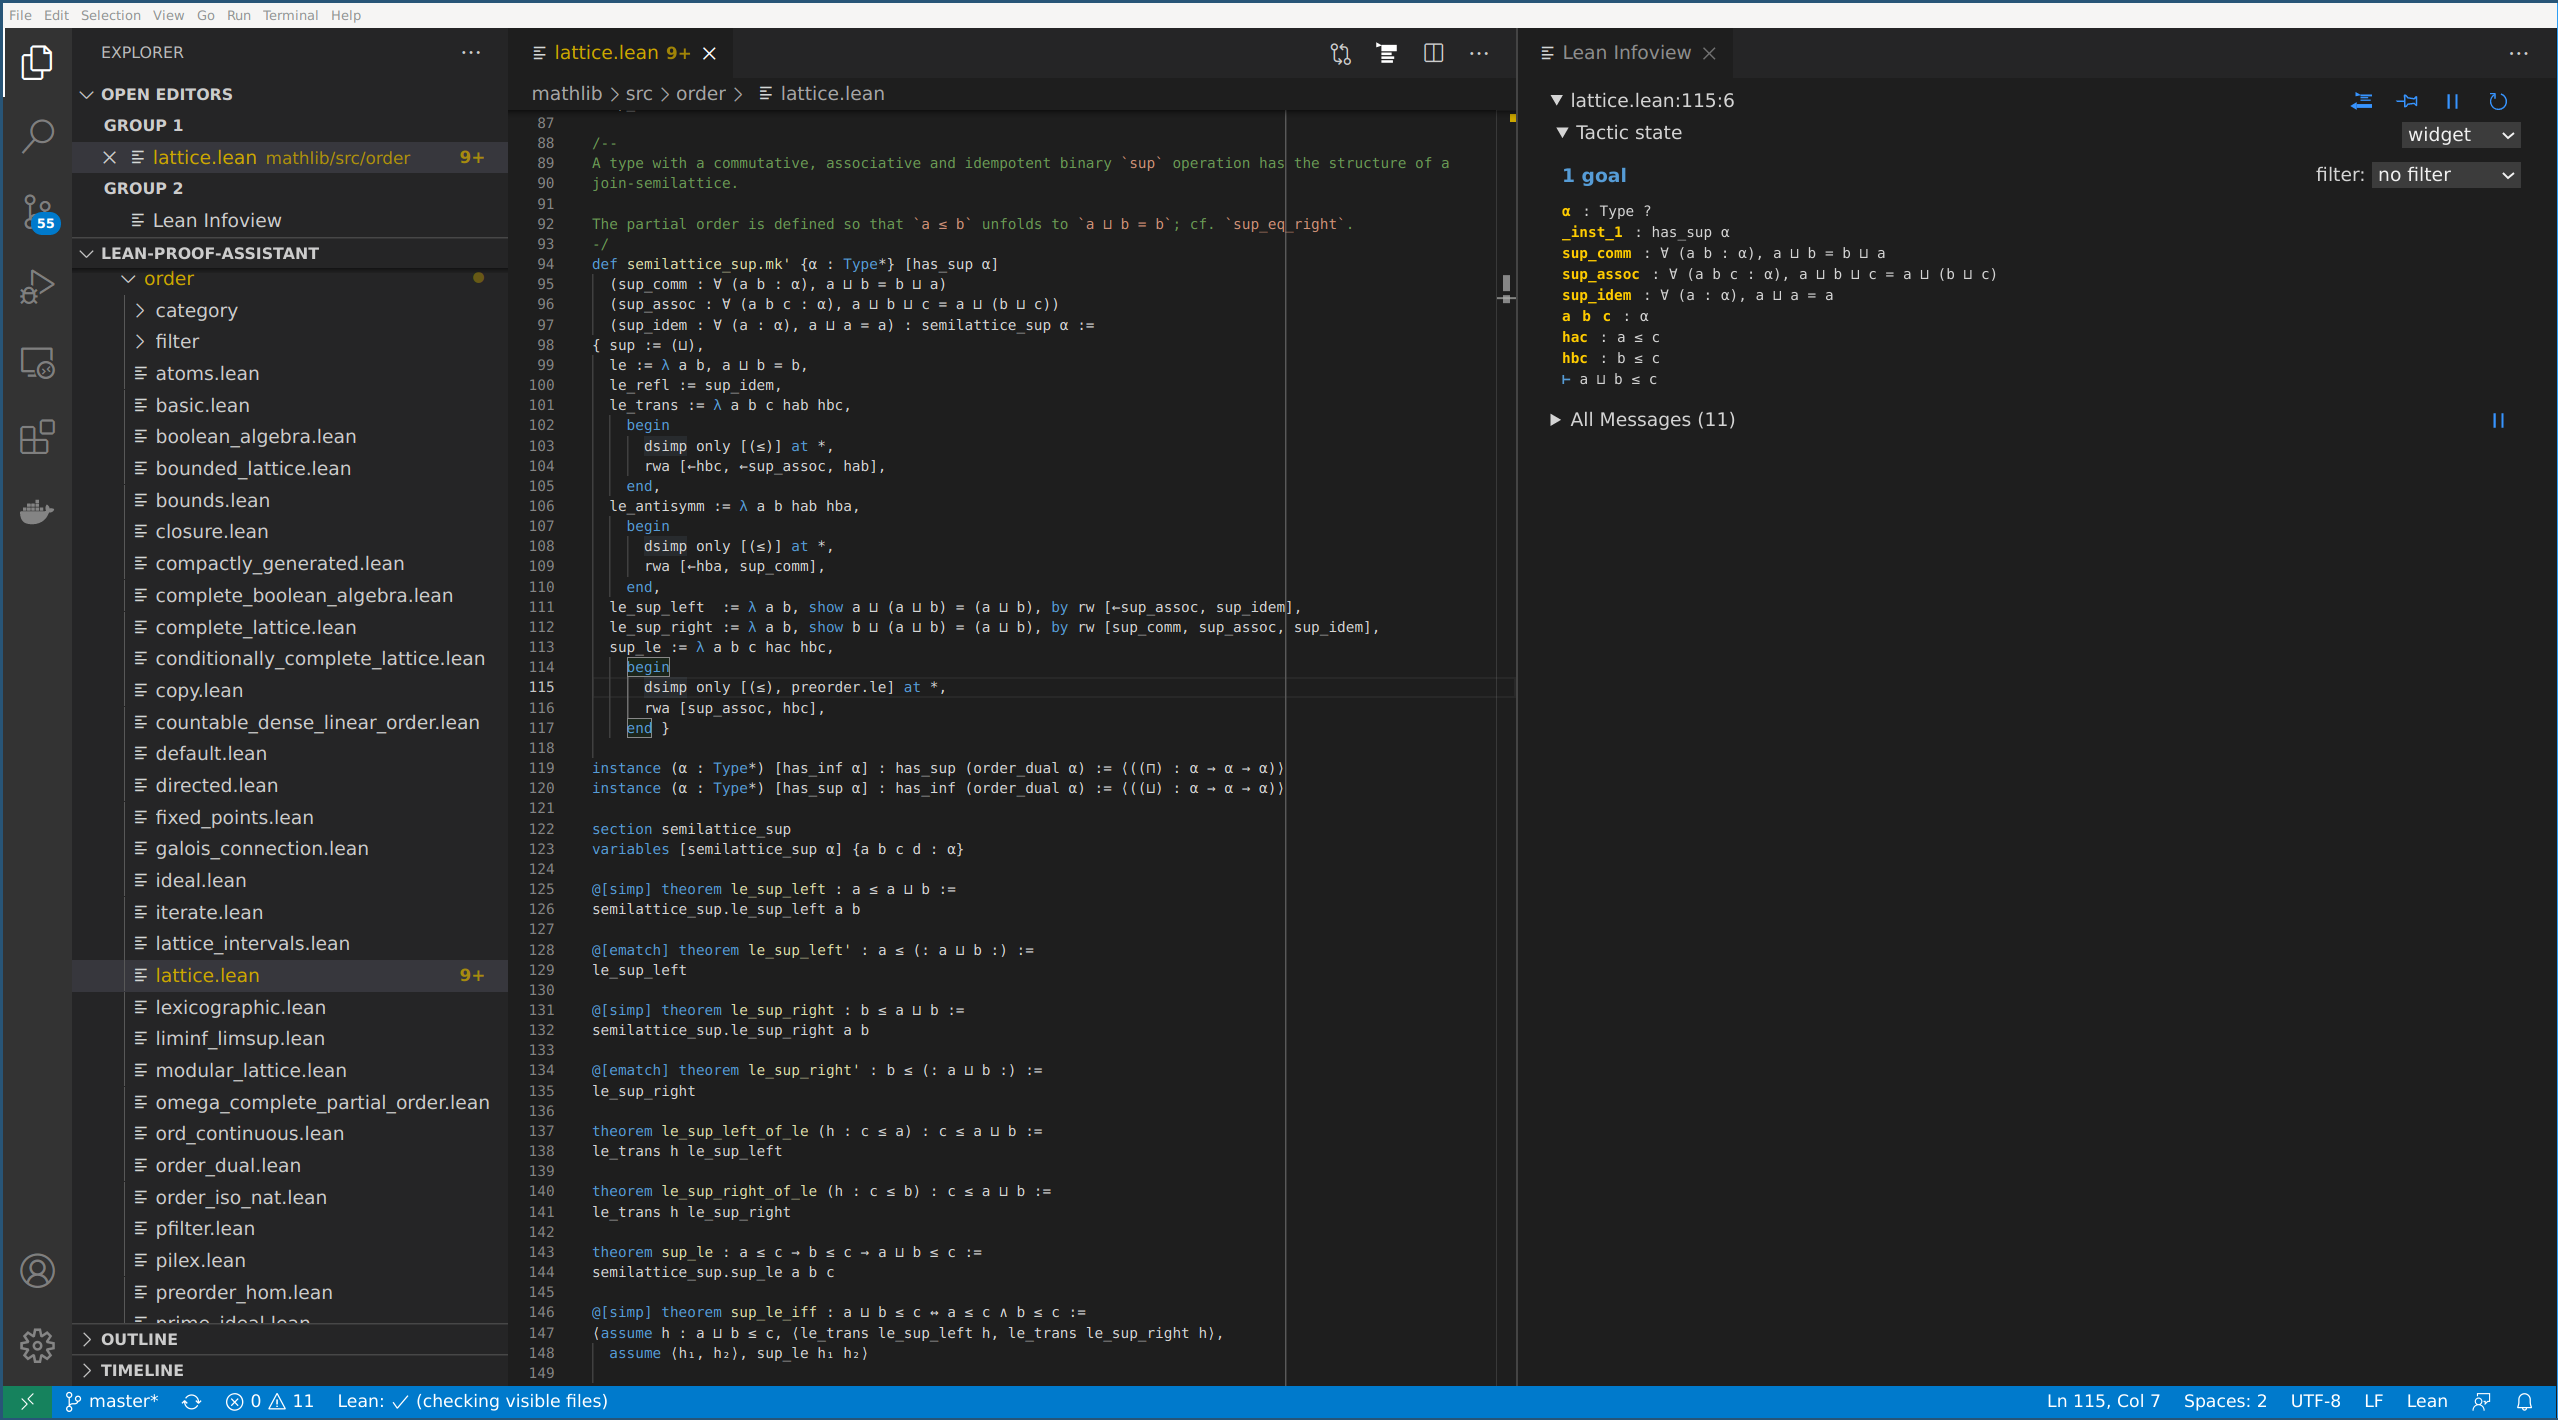
\includegraphics[scale=0.25]{vscode_printscreen.png}
        \caption{Vývojové prostredie}
    \end{figure}
\end{center}
    V pravom okne \emph{Lean infoview} je možné vidieť premenné s ich prislúchajúcimi
typmi a v prípade dôkazu aj formulu ktorú je potrebné dokázať za znakom $\vdash$.
    Okrem toho poskytuje okno aj výstup zo zabudovaných príkazov prostredia
ako \emph{print} alebo \emph{reduce} ktoré rozoberieme neskôr.
    V prípade že sa nachádzame v taktickom móde okrem zavedenia nových predpokladov
alebo transformácie existujúcich je možné vidieť aj zmenu cieľa a podcieľov
napríklad v prípade že sme sa dostali k dôkazu vymenovaním prípadov.
\section{$\lambda$-kalkulus}
    Pred predstavením techník dokazovania je nutné sa oboznámiť s prvkami funkcionionálneho
programovania v Leane.
    Výpočtový model jednoduchého $\lambda$-kalkulu je z programovacích paradigiem najbližšie práve funkcionálnemu spôsobu programovania.
V nasledujúcej časti predstavujeme základy funkcionálneho programovania spolu
    s typmi a nástrojmi Lean-u na vývoj a menežment priestor mien.
\subsection{Konštanty, aplikácie}
    Deklarácia konštanty zavádza do systému novú deklaráciu bez definície.
    Z tohto dôvodu sa ich pri rozvoji teórie snažíme vyhýbať.
    V nasledujúcich príkladov budeme pracovať s prirodzenými a celými číslami
ktorých štruktúry sú súčasťou kontextu bez nutnosti ich importovať.
\begin{lstlisting}
constant m : nat
\end{lstlisting}
    Hovorí o deklarovaní konštanty $m$ ktorej typ je \emph{nat}.
    Alternatívny zápis pre prirodzené číslo je pomocou sekvencie \emph{\textbackslash nat}
alebo \emph{\textbackslash N} ktorú skonvertuje leanovské rozšírenie na znak $\mathbb{N}$.
    Vstavaný príkaz ktorý poskytuje typ výrazu zadaného na argumente je \emph{\#check}:
\begin{lstlisting}
#check m
\end{lstlisting}
    Mriežka na začiatku príkazu značí zabudovaný príkaz.
    V tomto prípade je to triviálne tak ako bola konštanta zadefinovaná s výstupom
v informačnom okne:
\begin{lstlisting}
m : ℕ
\end{lstlisting}
    Pre zadefinovanie viacerých konštánt jedným príkazom a nie len v tomto prípade
existuje plurálna verzia príkazu \emph{constants}.

    Definícia konštanty typu funkcie medzi prirodzenými číslami vyzerá nasledovne:
\begin{lstlisting}
constant f : ℕ → ℕ
constant h : ℕ -> ℕ -> ℕ
\end{lstlisting}
    Aplikácia funkcie sa notačne podobá aplikácii v $\lambda$-kalkule kde argument
jednoducho pripíšeme za funkciu:
\begin{lstlisting}
#constants m n : ℕ

#check f m
#check h m
#check h m n
\end{lstlisting}
    Zatiaľ čo v prvom prípade dostaneme typ $\mathbb{N}$ v druhom prípade
$\mathbb{N} \to \mathbb{N}$ a v treťom vidíme aplikáciu na funkciu kde bude výsledným
typom znova jednoduchý typ $\mathbb{N}$.
    Aplikácia je asociatívna z ľavej strany a  preto je nasledujúci výraz potrebné 
uzátvorkovať napravo inak dostávame typový error pre funkciu $g$ ktorá očakáva 
celé číslo a nie typ funkcie f.
\begin{lstlisting}
constant f : ℕ → ℤ
constant g : ℤ → ℕ
constant a : ℕ

#check g (f a)
\end{lstlisting}
    Číselné konštanty má v leane typ $\mathbb{N}$.
\begin{lstlisting}
#check 5
#check (-5 : ℤ)
\end{lstlisting}
    Pri deklarácii záporného čísla je tak nutné už explicitne uviesť typ.
Nasledujúce príklady ilustrujú okrem funkcie $+$ aj implicitnú konverziu medzi typmi.
\begin{lstlisting}
#constants (m : ℕ) (n : ℤ)

#check 1 + 2
#check m + 1
#check n + 1
#check n + m
#check m + n
\end{lstlisting}
    V prípade prvého príkladu dostávame typ $\mathbb{N}$ pre nespracovaný výraz pre
ktorý by sme mohli očakávať výsledok $3$.
    Pre druhý a tretí výraz dostávame typy definovaných konštánt.
    Pri treťom výraze je vhodné si uvedomiť už implicitnú konverziu prirodzeného
čísla na celé.
    Konverzia je ešte viac zrejmá pri štvrtom výraze kde výsledným typom je
$\mathbb{Z}$.
    Prekvapivo z piateho výrazu dostávame v informačnom okne chybový výstup.
    Za neschopnosťou dostať typ stojí nedefinovaná konverzia z celých do prirodzených
čísel.
    Za vysvetlením stojí spôsob akým pracuje preťaženie infixového operátora $+$
podobným spôsobom ako pre triedy v jazyku $c++$ alebo $python$. Štvrtý a piaty
výraz je tak možné prepísať aj do tvaru:
\begin{lstlisting}
#check n.add(m)
#check m.add(n)
\end{lstlisting}
    Pretože znak $+$ je preťažením funkcie \emph{add} nad štruktúrou množiny daných
čísel.
\subsection{Funkcie}
    V predchádzajúcej sekcii sme si ukázali explicitný typ ktorý bol funkciou prirodzenými
číslami ktorý bol typu $\mathbb{N} \to \mathbb{N}$ alebo $\mathbb{N} \to \mathbb{N} \to \mathbb{N}$.
V Lean-e definujeme anonymnú funkciu alebo $\lambda$-výraz nasledovne.
\begin{lstlisting}
#check λ x, x + x
\end{lstlisting}
    Typ argumentu x je odvodený z výrazu ktorý na funkciu aplikujeme.
    Pre korektnú aplikáciu musí mať typ aj definovanú funkciu sčítania.
    Ak by sme chceli obmedziť argument len na konkrétny typ robíme to podobne ako
pri definovaní konštanty. Potom aplikácia
\begin{lstlisting}
#check (λ (x : ℕ), x + x) (m : ℤ)
\end{lstlisting}
je už typovou chybou pri ktorej nám informačné okno hlási
\begin{lstlisting}
type mismatch at application
  (λ (x : ℕ), x + x) m
term
  m
has type
  ℤ
but is expected to have type
  ℕ
\end{lstlisting}
    Uvedieme si zopár príkladov výpočtovo ekvivalentných funkcii obvodu obdĺžnika typu
$\mathbb{N} \to \mathbb{N} \to \mathbb{N}$.
\begin{lstlisting}
#check λ (x : ℕ) (y : ℕ), (x + x) + (y + y)
#check λ (x y : ℕ), (x + x) + (y + y)
#check λ (x : ℕ), λ (y : ℕ), (x + x) + (y + y)
\end{lstlisting}
    Všetky tri príklady sú ekvivalentné z pohľadu typov a predstavujú iný spôsob
zápisu.
    Funkcia v ktorej neuvedieme typ argumentu je polymorfnou.
\begin{lstlisting}
#check λ x y, x + x + y + y
\end{lstlisting}

    V prípade že by sme chceli získať hodnotu z výrazu použijeme príkaz \emph{\#eval},
alebo \emph{\#reduce}. \emph{Reduce} na rozdiel od \emph{eval} pri vykonávaní používa
jadro na získanie typu a je tak menej efektívnym.
\begin{lstlisting}
#eval (λ (x y : ℕ), (x + x) + (y + y)) 2 3
\end{lstlisting}
    Aplikácia nám dáva výsledok $10$ ktorý je očakávanou hodnotou.

    Pre pomenovanie alebo zadefinovanie takejto funkcie používame príkaz \emph{def}
ktorej tvar v najjednoduchšej podobe má tvar:
\begin{lstlisting}
def meno_definicie (argument_1 : typ) (argument_n : typ) :
    typ_navratovej_hodnoty 
:=
    telo funkcie
\end{lstlisting}
V prípade definície štvorca aj s jeho výpočtom
\begin{lstlisting}
def obvod_stvorca (x : ℕ) (y : ℕ) : ℕ := x + x + y + y

#eval obsah_stvorca 3 5
\end{lstlisting}

    Kľúčové slovo \emph{def} ktoré používame je funkčne bez funkčného roziedlu možné
zameniť za \emph{theorem}, \emph{lemma}. V prípade že chceme uviesť iba príklad
kde meno by pôsobilo nadbytočne používame slovo \emph{example}.

\subsection{Typy}
    Doteraz sme uvažovali len s typmi množiny prirodzených a celých čísel
ktoré predstavujú na pozadí Leanu konkrétne definovanú štruktúru.
    Typovanie v Lean-e ale podporuje zavedenie nového abstraktného typu ktorý patrí univerzu(universe).
    Zavedenie týchto univerz je motivované problémom analogickým s Russelovým paradoxom 
a teda či množina všetkých množín obsahuje samú seba.
    V teórii typov sa jedná o Girardov paradox.
    Hierarchia týchto univerz je usporiadaná od 0 čo je univerzum tvoriace najjednoduchšie
typy takže \emph{Type} alebo aj \emph{Type 0} je potom typom \emph{Type 1} ktorý
je typom \emph{Type 2}.

    Špeciálne postavenie v typoch majú tvrdenia označujeme \emph{Prop} ktorého
typom sú všetky dôkazy.
    Sú postavené v hierachii oddelené na najnižšej úrovni a teda \emph{Prop} je 
typu \emph{Type}.
    Univerzum do ktorého patrí \emph{Prop} označujeme \emph{Sort} čo je len 
alias.
Platí vzťah \emph{Sort u + 1} = \emph{Type u}.

V tejto práci a ani vo väčšine práce s Leanom nie je potrebné využívať hierachiu
    typov sofistikovanejším ako prezentovaným spôsobom.
\begin{lstlisting}
universe u v

constant (a : Typu u) (b : Type v)
\end{lstlisting}
Druhou možnosťou je využiť substitučnú syntax kde \emph{*} znamená pre ľubovoľné univerzum
a v prípade \emph{\_} necháme doplniť typ automaticky Lean-om.
\begin{lstlisting}
constant f : Type _ → Type _
constant g : Type

#check f g
\end{lstlisting}
    Kontrola typu aplikácie nám vypíše typ \emph{Type u\_1} čo je spôsob Lean-u označovať
ešte neurčený typ bez konkrétneho univerza.
\subsection{Premenné}
    V prípade že sa snažíme definovať viacero funkcií s rovnakými argumentami alebo
používať objekt ktorého typ je vyjadrený komplikovanejším zápisom je vhodné si
zápis zjednodušiť premennými.
    Z inak na pohľad komplikovaného zápisu
\begin{lstlisting}
universes u v

def kompozicia (α : Type u) (β : Type v) (f : α → β) (g : β → γ) (x : α) :
    α
:=
    g (f x)
\end{lstlisting}
    tak dostávame.
    Premenné vstupujú do predpokladov definícii len tam kde sú použité v jej tele.
\begin{lstlisting}
universes u v z

variable α : Type u
variable β : Type v
variable γ : Type z

def kompozicia (x : α) (f : α → β) (g : β → γ) : α := g (f x)
\end{lstlisting}
    Vstupné argumenty dokonca môžeme vynechať úplne, v niektorých prípadoch to ale
môže byť kontraproduktívne z dôvodu orientácie pri rozsiahlych zápisoch v editore.
\begin{lstlisting}
variables (f : α → β)
          (g : β → γ)

def kompozicia : α := g (f x)
\end{lstlisting}
Pre doplnenie dodávame že nie je nutné ani definovať návratový typ $\alpha$
    respektíve $\beta$, explicitné určenie návratového typu je ale vhodné nie len
    pre čitateľa ale aj pre overenie správnosti výsledného typu.
\subsection{Kontext, priestor mien}
    Pre ovládanie menného priestoru a kontextu existujú v Lean-e rôzne mechanizmy
z ktorých si popíšeme len tie najdôležitejšie.
    Najjednoduchším je súbor, ktorého definície, konštanty a premenné vstupujú do
kontextu pri deklarácii a na konci súboru zaniknú.
    Import obsahu iných súborov sa robí jednoduchým príkazom \emph{import} ktorý
musí byť deklarovaný na začiatku súboru. V súborovej hierachii sa potom od najvyššej
úrovne v jednej z vyhľadávaných ciest vnoríme cez bodku.
\begin{lstlisting}
import order.lattice
\end{lstlisting}
    Sa snaží nájsť priečinok \emph{order} so súborom \emph{lattice.lean}.
    V aktuálnej verzii Lean-u v čase písania práce sa dá zistiť zoznam prehľadávaných
ciest prepínačom \emph{path} priamo programu \emph{lean}.

    Deklarácie premenných definované v argumetnoch definície prepisujú vonkajší kontext.
    V prípade žeby sme chceli rozdeliť kontext súboru na menšie sekcie jednoduchým
nástrojom je dvojica \emph{section nazov\_sekcie}, \emph{end nazov\_sekcie}.
\begin{lstlisting}
section prirodzene_cisla
  variable α : ℕ
end prirodzene_cisla

section cele_cisla
  variable α : ℤ
end cele_cisla
\end{lstlisting}
    Používanejším je menný priestor \emph{namespace nazov} ktorý po zadefinovaní ponúka
možnosť opätovného zavedenia kontextu a vnorenie podobne ako rovnomenný mechanizmus
v jazyku C++.
\begin{lstlisting}
universe u

namespace skryty

  variable (α : Type u)
  namespace priestor
    def identita (a : α) : α := a
  end priestor
end skryty

#check skryty.priestor.identita

open skryty.priestor

#check identita
\end{lstlisting}
\section{Dokazovanie}

    K dokazovaniu v Leane je možné pristupovať viacerými spôsobmi.
    Po poskytnutí dôkazu už vnútorne Lean-u nezáleží na spôsobe akým bolo tvrdenie
dokázané.
    Prvým spôsobom je priamočiara konštrukcia typu pomocou funkcií.
    Druhým spôsobom je spätné dokazovanie ktoré využíva taktický mód za pomoci
sady príkazov upravujúcich cieľ a s pomocou poloautomatizácie.
    V leanovskej komunite je preferovaný práve druhý spôsob hoci pre jednoducho
dokázateľné tvrdenia stačí a je využívaná aj dopredná verzia.

\subsection{Dopredné dokazovanie}
    Dôkaz zostavený len z $\lambda$-funkcií ktoré transformujú argumenty
na výsledný typ je pri zložitejších dôkazoch ťažko čitateľný.
    Pre lepšiu čitateľnosť poskytuje Lean nástroje ktoré sa snažia konštruovať dôkazy tak
aby boli čitateľné ako tie klasické.
\begin{lstlisting}
variables p d : Prop

def plati_predpoklad : p → d → p := λ hp : p, λ hd : d, hp
\end{lstlisting}
    Predchádzajúci príklad je možné prepísať do čitateľnejšej verzie
\begin{lstlisting}
def plati_predpoklad : p → d → p :=
  assume hp : p,
  assume hd : d,
  show p, from hp
\end{lstlisting}
Pre lepšiu predstavu toho čo sa deje na pozadí Lean poskytuje výstup:
\begin{lstlisting}
pq: Prop
hp: p
hq: q
⊢ p
\end{lstlisting}
    Funkcie sú asociatívne zprava $p \to ( d \to p )$.
    Tvrdenie hovorí "ak platí $p$, potom z $d$ vyplýva $p$".
\begin{itemize}
    \item Predpokladajme hp,
    \item a predpokladajme hd,
    \item potom vieme ukázať že platí p z predpokladu hp.
\end{itemize}
    O čosi zložitejším príkladom je tvrdenie že ak platí $p$ konjukcia $q$ tak potom
platí $q$ konjukcia $p$.
\begin{lstlisting}
def symetria_konjukcie : p ∧ q → q ∧ p :=
  assume hpq : p ∧ q,
    have hp   : p     := and.left  hpq,
    have hq   : q     := and.right hpq,
    have hqp  : q ∧ p := and.intro hq hp,
  show q ∧ p, from hqp
\end{lstlisting}
    Konjukciu v editore je možné napísať cez \emph{\textbackslash and}.
    Ak sa pozrieme na typ konjukcie a funkcií ktoré sme dostali cez príkaz check.
    Dostaneme výstup:
\begin{lstlisting}
and : Prop → Prop → Prop
and.left : ?M_1 ∧ ?M_2 → ?M_1
and.right : ?M_1 ∧ ?M_2 → ?M_2
and.intro : ?M_1 → ?M_2 → ?M_1 ∧ ?M_2
\end{lstlisting}
    Toto intuitívne korenšponduje s tým čo od týchto funkcií očakávame.
    Tento dôkaz je rozšírený o príkaz have ktorý vytvára predpoklad z existujúcich.
    V poslednej fáze dôkazu je interaktívny výstup:
\begin{lstlisting}
pq: Prop
hpq: p ∧ q
hp: p
hq: q
hqp: q ∧ p
⊢ q ∧ p
\end{lstlisting}

\subsection{Spätné dokazovanie}

    V doprednom dokazovaní sme sa snažili transformovať predpoklady tak aby na konci
bol výsledkom dôsledok.
    Ako evokuje názov v spätnom dokazovaní sa snažíme transformovať cieľ tak aby sme
sa dostali k jednému z predpokladov.
    Pre tento účel existuje v Lean-e špeciálny spôsob dokazovania ktorý nazývame taktický
mód.
    Na rozdiel od dopredného dokazovania je nutné ovládať väčšiu sadu príkazov ktoré
priamo transformujú cieľ.
    Dokazovanie je tak užšie prepojené s interaktívnym prostredím a pripomína tak hru.
    Ďalšou výhodou tohto dokazovania je možnosť využitie umelej inteligencie pri vyhľadaní
dôkazu.
    Takýto prístup je obzvlášť užitočný napríklad v prípade že musíme dokázať identitu
ktorej dôkaz je prácny, a tvorí ho veľa za sebou nasledujúcich využití iných
identít ako napríklad využitie komutativity alebo asociativity.
    Užšie prepojenie s prostredím a automatizácia vyhľadania dôkazu tohto módu ale
ide na úkor priamej čitateľnosti.
    Pre úplnosť dopĺňame že v taktickom móde nie je nutné transformovať cieľ a je možné
využiť aj konštrukcie dopredného dôkazu.

    Pre dokazovanie v taktickom móde používame konštrukciu ktorá je ohraničená
kľúčovými slovami \emph{begin} a \emph{end}.

\begin{lstlisting}
def symetria_konjukcie : p ∧ q → q ∧ p :=
  begin
    intro h,
    cases h with p q,
    split,
    exact q,
    exact p
  end
\end{lstlisting}

    Dôkaz začína zavedením predpokladu z implikácie k ostatným o ktorých tvrdíme
že sú pravdivé príkazom \emph{intro} a rozdelením konjukcie príkazom \emph{cases}
s argumentom zavedenej konjukcie a ich explicitným pomenovaním.
    Výstup v informačnom okne potom obsahuje.

\begin{lstlisting}
pq: Prop
p: p
q: q
⊢ q ∧ p
\end{lstlisting}

Príkazom \emph{split} potom rozdelíme cieľ na podciele kde sa snažíme dokázať
ľavú a pravú stranu ktorú vidíme v informačnom okne ako:

\begin{lstlisting}
2 goals
pq: Prop
h_left: p
h_right: q
⊢ q
pq: Prop
h_left: p
h_right: q
⊢ p
\end{lstlisting}

Dôkaz potom uzatvoríme príkazom \emph{exact} ktorý ukáže na jeden z predpokladov
    s rovnakým typom ako cieľ.

\section{Abstraktné štruktúry v Lean-e}
    V matematike a tak isto aj v programovaní sa často vyskytujú objekty
nad ktorými je možné vykonávať operácie bez ohľadu na ich obsah pri splnení
určitých podmienok.
    V matematike hovoríme o štruktúrach, ktoré majú striktnú definíciu v programovaní
sa dá voľne hovoriť o triedach.
    Matematické štruktúry v Lean-e su navrhované práve pomocou mechanizmu tried,
pričom definícii triedy zodpovedá štruktúra spĺňajúca z definíce vyplývajúce podmienky.
    Potom inštanciou triedy môže byť znova štruktúra ktorá je definovaná na užšej množine
znova spĺňajúcej podmienky, príkladom je vzťah grupy a podgrupy alebo
priestoru a podpriestoru.
    Druh hierachie potom tvorí možnosť rozširovania tried pri ktorých spĺňa okrem
podmienok pôvodnej štruktúry aj ďalšie ktoré ju obohacujú.
    Príkladom využitia môže byť pologrupa ktorá je množinou s asociatívnou operáciou
a monoidom, čo je pologrupa s jednotkou.
\subsection{Induktívne štruktúry}

    Induktívne štruktúry predstavujú notačne silný nástroj pre definíciu objektov
medzi ktorými je jednoduchá asocioácia.
    Jednoduchým príkladom je zoznam kde asociáciou medzi prvkami tvorí vzťah
usporiadania.
    Komplikovanejší klasický príklad tvoria stromové štruktúry tvoriace uzly
s viacerými nasledovníkmi.
    V matematike sa s indukciou stretávame pri definícii prirodzených čísel
cez Peanove axiómy.
    Dve z týchto axióm hovoria:
\begin{itemize}
    \item 0 je číslo
    \item Ak $a$ je číslo potom nasledovník $a$ je tiež číslo.
\end{itemize}
    Prvé pravidlo hovorí o základnom prípade, v prípade zoznamu alebo stromu prázdny
zoznam respektíve strom.
    Implementácia prirodzených čísel pomocou indukčnej štruktúry by mohla vyzerať
nasledovne:
\begin{lstlisting}
inductive prirodzene : Type
  | nula        : prirodzene
  | nasledovnik : prirodzene → prirodzene
\end{lstlisting}
    Za kľúčovým slovom inductive nasleduje názov a sada konštruktorov s návratovými
typmi.
    Už z názvu vyplýva súvislosť s dôkazom s matematickou indukciou kde platnosť
nejakého tvrdenia $P(n)$ pre všetky prirodzené čísla sa dokazuje pre
\begin{itemize}
    \item $P(0)$, t.j. základný prípad
    \item $\forall n \in \mathbb{N}, P(n) \implies P(n+1)$, indukčný krok
\end{itemize}
    Pre tento typ dôkazu existuje v Leane v taktickom móde príkaz \emph{induction}.
\begin{lstlisting}
example : 5 * n = 4 * n + n :=
    begin
      induction n with d hd,
      ...
    end
\end{lstlisting}
    Po príkaze induction sa informačnom nachádzajú dva ciele pre obe konštruktory
prirodzených čísel \emph{nat.zero} a \emph{nat.succ} podobne ako v našej uvedenej
štruktúre a základnému prípadu a tvrdeniam matematickej indukcie dokazujúcej platnosť
$P$.
\begin{lstlisting}
case nat.zero
⊢ 5 * 0 = 4 * 0 + 0

case nat.succ
d: ℕ
hd: 5 * d = 4 * d + d
⊢ 5 * d.succ = 4 * d.succ + d.succ
\end{lstlisting}

    V príklade ktorý sme uviedli sú znamienka $+$ a $*$ ktoré používame
v operáciach nad typom našej induktívnej štruktúry.
    Výsledkom oboch binárnych operácii je znova prirodzené číslo.
    Podľa predpokladov typ ktorý prislúcha ich definícii je
$prirodzene \to prirodzene \to prirodzene$.
    Jednou z výhod indkučne definovaných štruktúr je jednoduchosť definovania
rekurzívnych funkcií ktoré operujú nad týmito štruktúrami.
\begin{lstlisting}
variables (a b: prirodzene)

open prirodzene

def sucet : prirodzene → prirodzene → prirodzene
  | a    nula         := a
  | a (nasledovnik b) := nasledovnik (sucet a b)
\end{lstlisting}
    V tomto prípade znamená notácia $|$ prípad v ktorom sa snažíme nájsť zhodu
s poskytnutým argumentom a návratový typ.
    V treťom prípade ide o rekurzívne pravidlo ktoré z argumentu $b$ vytvorí jedo
predchodcu.
    Celé pravidlo potom vráti nasledovníka zo súčtu prvého argumentu a predchodcu
druhého.
    Rekurzia tak prenáša vlastnosť nasledovania z prvého na druhý argument až
sa argumenty nezhodujú s prvým pravidlom a teda argument už nemá predchodcu.
    Pre úplnosť dodávame aj technický detail definovania znamienka $+$ ako volania
funkcie súčtu:
\begin{lstlisting}
local infix ` + ` := sucet
\end{lstlisting}

\subsection{Jednoduché štruktúry}
    V prípade že by jeden z konštruktorov neobsahoval typ ktorý poskytuje funkciu
medzi typmi samotnej štruktúry, ide o obyčajnú štruktúru.
    Ich využitie je najmä pri definovaní tých matematických a v lean-e majú
špeciálnu syntax.
    V príklade uvádzame ekvivalentné spôsoby definovania štruktúr.
\begin{lstlisting}
structure vector :=
  mk :: (x y: ℝ)

structure vector₂ :=
  (x : ℝ)
  (y : ℝ)
\end{lstlisting}
    Vytváranie objektov danej štruktúry má explicitné priradzovanie prvkom
podľa názvov v prípade jednoduchých štruktúr je vhodnejšie priradzovanie na
základe poriadia z definície šturktúry.
\begin{lstlisting}
def v₂ : vector₂ :=
  {
    x := 10.5,
    y := 13.7,
  }

#check (⟨10.5, 13.7⟩ : vector)
\end{lstlisting}
    K jednotlivým prvkom štruktúry pristupujeme cez bodku:
\begin{lstlisting}
#eval v.x
\end{lstlisting}
    tak vracia hodnotu 10.5.
    Pre modelovanie hierarchie kde jedna štruktúra rozširuje druhú používame
kľúčové slovo \emph{extends}.
    Rozšírenie našej štruktúry o ďalšiu dimenziu vyzerá nasledovne:
\begin{lstlisting}
structure vector₃ extends vector₂ :=
  (z : ℤ)

def ∨₃₁ : vector₃ :=
  { x := 1, y := 2, z := 3}
\end{lstlisting}
    V prípade že chceme vytvoriť objekt z rozšírenej štruktúry a máme k dispozícii
jeho podkladový je často využívaná notácia.
\begin{lstlisting}
def ∨₃₂ : vector₃ :=
{
    z := 10, ..v₂
}
\end{lstlisting}
    Závislostné typy predstavujú mechanizmus parametrizácie štruktúr a definícii
na základe poskytnutého typu.
    V prípade nášho vektora by sme túto vlastnosť mohli využiť ak by sme chceli
zúžiť množinu z ktorej pochádza náš vektora len na celé čísla.
\begin{lstlisting}
structure vector { α : Type u } :=
  (x : α)
  (y : α)
  (z : α)

def v₁ := (⟨10, 13, 3⟩ : vector)
def v₂ := (⟨(-10 : ℤ), 13, 3⟩ : vector)

#check v₁.z
#check v₂.z
\end{lstlisting}
    Pri prvej kontrole sme dostali typ $\mathbb{N}$.
    V druhom prípade je ale $z$-tová zložka vektora $v_{2}$ typu $\mathbb{Z}$.
    Nedostatkom uvedeného príkladu je že množina $\mathbb{Z}$ obsahuje
množinu $\mathbb{N}$.
    Príkladom ktorý lepšie ilustruje možnosti využitia sú matematické štruktúry,
ktoré sú definované na množinách ktoré môžu obsahovať objekty ľubovoľného typu.
\begin{lstlisting}
variables { T : Type* } ( A : štruktúra₁ T ) ( B : štruktúra₂ T)
\end{lstlisting}
    Takáto definícia premenných $A$ a $B$ zase zaručuje že množina na ktorých sú
štruktúry definované je rovnakého typu.
    V prípade že by sme výraz uzátvorkovali do obyčajných zátvoriek použili v
definícii:
\begin{lstlisting}
lemma ( T : Type* ) ( A : štruktúra₁ T ) ( B : štruktúra₂ T) : Type :=
begin
    ...
end
\end{lstlisting}
    Musíme pri použiti alebo zavolaní poskytnúť aj prvý argument.
    Z tohto dôvodu sa tejto konštrukcii hovorí aj implicitný argument.
\begin{lstlisting}
lemma { T : Type* } ( A : štruktúra₁ T ) ( B : štruktúra₂ T) : Type :=
begin
    ...
end
\end{lstlisting}
Typy na ktorých sú definované argumenty závisia od implictného.
\subsection{Typové triedy}
    Typové triedy poskytujú mechanizmus pomocou ktorého zlučujeme rozdielne štruktúry
s rovnakou vlastnosťou do tried.
    Príkladom môžu byť mať vlastnosť usporiadania, mať reprezentanta alebo
byť grupou.
    Po zadefinovaní triedy potom štruktúru priradíme do tried inštancovaním.
    Inštancovanie pre štruktúry potom býva odlišné v závislosti definície štruktúry.
    Vykonávanie dôkazov nad typovou triedou potom umožňuje zredukovať množstvo definícii.
    Nad našimi definíciami vektorov môžeme definovať dĺžku.
\begin{lstlisting}
class norm (α : Type u) :=
  (length : α → ℝ)
\end{lstlisting}
    Potom k definíciam štruktúr pridáme inštancie.
\begin{lstlisting}
instance vector₂_norma : norma vector₂ :=
 { length := λ (v : vector₂), sqrt(v.x * v.x + v.y * v.y) }

instance vecotr₃_norma : norma vector₃ :=
 { length := λ (v : vector₃), sqrt(v.x * v.x + v.y * v.y + v.z * v.z) }
\end{lstlisting}
    Triedu potom využívame v definíciach uvedením do hranatých zátvoriek aj s
argumentom.
\begin{lstlisting}
variables { T : Type* } ( a : štruktúra₁ T ) ( b : štruktúra₂  T ) [ norma T ]
\end{lstlisting}
    Tento už komplikovanejší zápis hovorí o premenných $a$ a $b$ ktoré sú definované
na rovnakom type ktorý má definovanú alebo je inštancovaný dĺžkou.

\chapter{Teória čiastočného usporiadania}
    V tejto kapitole sa budeme snažiť ukázať možnosti Lean-u a využitie už existujúcich
definícii v mathlibe pre dokázanie viet týkajúcich sa teórie čiastočného usporiadania.
    Pre tento účel je v Lean-e možnosť definovania vlastností usporiadania, 
ktoré následne možno aplikovať na abstraktnú množinu objektov.
    Výsledný typ je potom odvodený na základe závislostných typov.
    Usporiadanie je jednoducho intuitívne pochopiteľná vlastnosť bez matematických
predispozícii.
    V každodennom živote porovnávame svoju výšku, čas, ktorý trval na vybehnutie do kopca
alebo aj číselne neohodnotené, subjektívne merateľné objekty ako ktorý album
od skupiny preferujem.
    Na otázky si potom vieme odpovedať "ja som vyšší", "zabehol si pomalšie" alebo
tieto "albumy sú neporovnateľné".
    Teória usporiadania sa snaží tieto vlastnosti formálne definovať a rozvíjať ďalej
otázkami ako,

\begin{itemize}
    \item Aké je horné celej množiny objektov?
    \item Existuje ohraničenie horné alebo dolné pre ľubovoľnú podmnožinu objektov?
    \item Ako vyzerá zobrazenie zachovávajúce usporiadanie?
\end{itemize}
    Pre stručnosť sa v rámci definícii obmedzíme len na definíciu relácie usporiadania,
čiže podmnožinu karteziánskeho súčinu dvoch množín.
\begin{definition}
    Majme množinu $P$, potom usporiadanie alebo čiastočné usporiadanie na množine
    $P$ je binárna relácia $\leq$ taká že, pre všetky $x,y,z \in P$
    \begin{itemize}
        \item $x \leq x$ reflexivita
        \item $x \leq y$ a $y \leq x$ implikuje $x = y$ antisymetria
        \item $x \leq y$ a $y \leq z$ impikuje $x \leq z$ tranzitivita
    \end{itemize}
\end{definition}
    Ideálnym nástrojom pre uvažovanie nad usporiadaním sú \emph{Hasseho} diagramy.
    Ako príklad uvádzame diagram "kocky".
\begin{figure}[!ht]
    \centering
    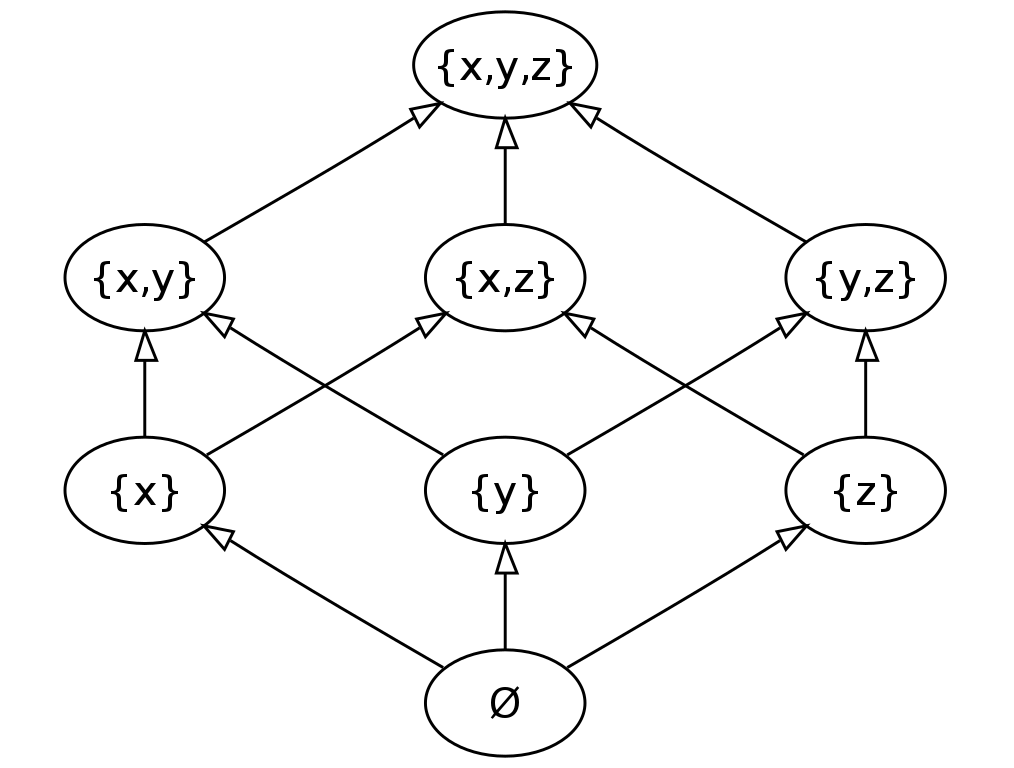
\includegraphics[scale=0.20]{cube.png}
    \caption{Usporiadania $\mathcal{P}(\{a,b,c\})$}
\end{figure}

    % TODO prerobit vetu % 
    Na obrázku je usporiadanie všetkých podmnožín trojprvkovej množiny $\{ a,b,c \}$
vzhľadom na kardinalitu podmnožín.
    Za porovnateľné považujeme len tie prvky, ktoré sú "pokryté" jednosmernou cestou 
cez orientované hrany grafu.

    V Leane je usporiadanie definované ako rozšírenie triedy predusporiadania, ktorá
je reláciou, ktorá nemá oproti čiastočnému usporiadaniu vlastnosť antisymetrie.

\begin{lstlisting}
class has_le       (α : Type u) := (le : α → α → Prop)
class has_lt       (α : Type u) := (lt : α → α → Prop)

class preorder (α : Type u) extends has_le α, has_lt α :=
(le_refl : ∀ a : α, a ≤ a)
(le_trans : ∀ a b c : α, a ≤ b → b ≤ c → a ≤ c)
(lt := λ a b, a ≤ b ∧ ¬ b ≤ a)
(lt_iff_le_not_le : ∀ a b : α, a < b ↔ (a ≤ b ∧ ¬ b ≤ a) . order_laws_tac)
\end{lstlisting}
    Čiastočné usporiadanie je potom rozšírením predusporiadania o vlastnosť antysymetrie.
\begin{lstlisting}
class partial_order (α : Type u) extends preorder α :=
(le_antisymm : ∀ a b : α, a ≤ b → b ≤ a → a = b)
\end{lstlisting}

\section{Zväz}
    Zväz je čiastočne usporiadaná množina, pre ktorú navyše platí, že pre každé 2 prvky $a, b$
vieme nájsť prvok $c$, ktorý je ich jedinečným najmenším horným, respektíve(\emph{supremum})
najväčším dolným ohraničením(\emph{infimum}).
    V prípade intervalu reálnych čísel je toto ohraničenie jednoducho predstaviteľné
ako bod ohraničujúce množinu na číselnej osi.
    Ak ide o čiastočné usporiadanie, názov je pre tieto ohraničenia prvkov
motivovaný zobrazením na grafe.
    \emph{Spojenie} $\sqcup, \vee$ pre supremum, respektíve \emph{priesek} $\sqcap, \wedge$ pre infimum.
    Popisnejším názvom pre zväz je preklad anglicky používaného názvu \emph{lattice}
"mriežka" tak isto motivovaná zobrazením takého usporiadania na grafe.
    Pri dokazovaní viet o zväzoch je často využívaná vlastnosť duality najmenšieho
horného a duálne najväčšieho dolného ohraničenie pre druhú polovicu dôkazu.
\begin{lstlisting}
class has_sup (α : Type u) := (sup : α → α → α)
class has_inf (α : Type u) := (inf : α → α → α)

infix ⊔ := has_sup.sup
infix ⊓ := has_inf.inf

class semilattice_sup (α : Type u) extends has_sup α, partial_order α :=
(le_sup_left : ∀ a b : α, a ≤ a ⊔ b)
(le_sup_right : ∀ a b : α, b ≤ a ⊔ b)
(sup_le : ∀ a b c : α, a ≤ c → b ≤ c → a ⊔ b ≤ c)

class semilattice_inf (α : Type u) extends has_inf α, partial_order α :=
(inf_le_left : ∀ a b : α, a ⊓ b ≤ a)
(inf_le_right : ∀ a b : α, a ⊓ b ≤ b)
(le_inf : ∀ a b c : α, a ≤ b → a ≤ c → a ≤ b ⊓ c)

class lattice (α : Type u) extends semilattice_sup α, semilattice_inf α
\end{lstlisting}

\section{Modulárne zväzy}

    V nasledujúcom úseku si ukážeme vetu týkajúcu sa špeciálneho typu zväzu s vlastnosťou
modularity a ukážeme si formálny dôkaz a jej implementáciu v Leane, ktorú si
podrobne rozoberieme.

    O zväze $L$ hovoríme, že je modulárny, v prípade, že má nasledujúcu vlastnosť.

\begin{equation*}
    (\forall x,y,z \in L) x \geq y \implies x \wedge ( y \vee z) = (x \wedge y) \vee z
\end{equation*}

    V Leane definovaný ako rozšírenie zväzu:

\begin{lstlisting}
class modular_lattice(α : Type u) extends lattice α :=
  (modular_law: ∀ (x u v : α ), (x ≤ u) → u ⊓ (v ⊔ x) = (u ⊓ v) ⊔ x )
\end{lstlisting}

    V nasledujúcom úseku si ukážeme vetu o izomorfizme pre modulárne zväzy a podrobne
si rozoberieme implementáciu jej dôkazu s obsahom prostredia v Leane.

\begin{theorem} \emph{Veta o izomorfizme pre modulárne zväzy}
Nech L je modulárnym zväzom a $a, b \in L$. Potom
    \begin{equation}
        \varphi_{b}: x \mapsto x \wedge b, x \in [a, a \vee b],
    \end{equation}
Je izomorfizmom medzi intervalmi $[a, a \vee b]$ a $[ a \wedge b, b]$.
Inverzným izomorfizmom je
    \begin{equation}
        \psi_{a}: y \mapsto y \vee a, y \in [a \wedge b, b].
    \end{equation}
\end{theorem}
\emph{Dôkaz}.
    Stačí ukázať, že $\varphi_{b}\psi_{a}(y) = y$ pre všetky $y \in [a \wedge b, b]$.
    Z duality potom vyplýva, že $\psi_{a}\varphi_{b}(x) = x$ pre všetky
$x \in [a, a \vee b ]$,
    Nech $y \in [ a \wedge b, b ]$, potom $\varphi_{b}\psi_{b} = ( y \vee b ) \wedge a$ 
a ak platí nerovnosť $b \geq y$ tak potom z modularity
    \begin{equation}
        \varphi_{b}\psi_{a}(y) =
        ( y \vee b ) \wedge a =
        y \vee ( b \wedge a) =
        y
    \end{equation}
    pretože
    \[
        \pushQED{\qed}
        y \geq a \wedge b. \qedhere
        \popQED
    \]

    Horeuvedený dôkaz je znázornený na nasledujúcom obrázku.

\begin{figure}[!ht]
    \centering
    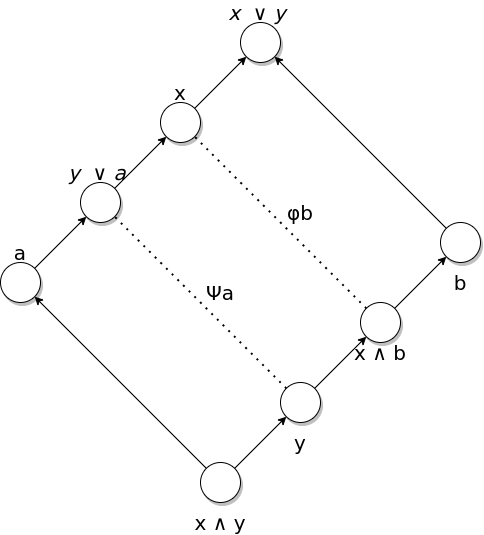
\includegraphics[scale=0.35]{modular_lattice_isomorphism.png}
    \caption{Izomorfizmus modulárneho zväzu}
\end{figure}
k
    V prípade formálneho dôkazu sme sa mohli v časti dôkazu odkázať na dualitu.
    Pri návrhu dôkazu v Leane musíme ukázať dôkaz z "oboch" strán. Najskôr uvedieme
hotový dôkaz vety:
\begin{lstlisting}
theorem modular_lattice_isomorphism { α: Type u } [ modular_lattice α ] { a b x : α}:
  x ≤ a →
  x ≥ b →
  x ≥ a ⊓ b →
  x ≤ a ⊔ b →
  a ⊓ ( b ⊔ x ) = x ∧ (a ⊓ x) ⊔ b = x
  :=
  begin
    intros h1 h2 h3 h4,
    split,
    {
      rw modular_lattice.modular_law,
      exact sup_eq_right.mpr h3,
      exact h1
    },
    {
      rw inf_comm,
      rw ← modular_lattice.modular_law,
      exact inf_eq_left.mpr h4,
      exact h2
    }
  end
\end{lstlisting}
    Začíname v taktickom móde ktorý je interaktívnou verziou dokazovania v Leane.
    Po zadaní prázdnej konštrukcie \emph{begin} a \emph{end}
    Interaktívne prostredie vyzerá nasledovne.
\begin{lstlisting}
α: Type u
_inst_1: modular_lattice α
abx: α
⊢ x ≤ a → x ≥ b → x ≥ a ⊓ b → x ≤ a ⊔ b → a ⊓ (b ⊔ x) = x ∧ a ⊓ x ⊔ b = x
\end{lstlisting}
    Prvým krokom dôkazu je presunutie predpokladov zo sledu implikácii do
prostredia pre ďalšiu prácu s nimi s označením $h1,h2,h3,h4$.
\begin{lstlisting}
α: Type u
_inst_1: modular_lattice α
abx: α
h1: x ≤ a
h2: x ≥ b
h3: x ≥ a ⊓ b
h4: x ≤ a ⊔ b
⊢ a ⊓ (b ⊔ x) = x ∧ a ⊓ x ⊔ b = x
\end{lstlisting}
    Cieľ potom pozostáva z konjukcie, kde v druhej časti máme výraz implicitne
ozátvorkovaný zľava.
    Výraz rozdelíme do dvoch podcieľov príkazom \emph{split}, a pre lepšiu
čitateľnosť ozátvorkujeme množinovými zátvorkami. Nachádzame sa v stave
\begin{lstlisting}
  begin
    intros h1 h2 h3 h4,
    split,
    {
    },
    {
    }
  end
\end{lstlisting}
v ktorom nám lean ukazuje prostredie, kde musíme dokázať ľavú časť konjukcie.
\begin{lstlisting}
⊢ a ⊓ (b ⊔ x) = x
\end{lstlisting}
Na cieľ použijeme z definície modulárneho zväzu vlastnosť modularity
\begin{lstlisting}
    (modular_law: ∀ (x u v : α ), (x ≤ u) → u ⊓ (v ⊔ x) = (u ⊓ v) ⊔ x )
\end{lstlisting}
a transformujeme prepíšeme cieľ cez príkaz
\begin{lstlisting}
rw modular_lattice.modular_law,
\end{lstlisting}
na nasledujúci, kde má $u \sqcap v$ vyššiu precedenciu
\begin{lstlisting}
⊢ u ⊓ v ⊔ x = x
\end{lstlisting}
    Nasledujúca transformácia vyžaduje znalosť už dokázaných definícií, ktoré
boli dokázané pre podkladové štruktúry. Použijeme nasledujúcu definíciu, ktorá vychádza
z kontextu \emph{semilattice\_sup}.
\begin{lstlisting}
% @ [simp] theorem sup_eq_right : a ⊔ b = b ↔ a ≤ b :=    / TODO NEZABUDNUT
%  le_antisymm_iff.trans $ by simp [ le_refl ]             / ODKOMENTOVAT
\end{lstlisting}
    Zaujímavosťou je, že si Lean dokáže substiuovať výraz $u \sqcap v$ za $a$ z uvedeného
výrazu. Pri použití vety dostávame ekvivalenciu, ktorá je definovaná ako štruktúra.
\begin{lstlisting}
structure iff (a b : Prop) : Prop :=
    intro :: (mp : a → b)
             (mpr : b → a)
\end{lstlisting}
Z tejto štruktúry použijeme implikáciu smerujúca doľava nasledovne:
\begin{lstlisting}
    exact sup_eq_right.mpr h3,
\end{lstlisting}
    Cieľ je teda transformovaný na:
\begin{lstlisting}
⊢ x ≤ a
\end{lstlisting}
čo je už uvedený predpoklad $h1$. Týmto sme dokázali jeden z podcieľov.
    V tejto chvíli by sme sa v literatúre mohli odvolať na dualitu výrazov.
    V Leane musíme poskytnúť dôkaz aj o druhom cieli. Ideme dokázať
\begin{lstlisting}
⊢ a ⊓ x ⊔ b = x
\end{lstlisting}
V tejto chvíli chceme znova použiť modularitu, leanu je, ale potrebné explicitne povedať,
    že chceme prepísať výraz nachádzajúci na pravej strane rovnosti pomocou symbolu
ľavej šípky.
\begin{lstlisting}
rw ← modular_lattice.modular_law,
\end{lstlisting}
    Použijeme duálnu vetu
    duálnu k \emph{sup\_eq\_right}.
\begin{lstlisting}
@[simp] theorem inf_eq_left : a ⊓ b = a ↔ a ≤ b
\end{lstlisting}
    a využijeme opačné predpoklady k predchádzajúcim $h2, h4$.
\begin{lstlisting}
{
    rw ← modular_lattice.modular_law,
    exact inf_eq_left.mpr h4,
    exact h2
}
\end{lstlisting}

    Po dokázaní druhého cieľa sme dokázali celú vetu. $\square$

\section{Podzväz}

    V rámci príspevku do knižnice \emph{mathlib} sme implementovali štruktúru
reprezentujúcu podzväz. Formálne je definovaný:

\begin{theorem}
    Nech $L$ je zväz. Množina $K \subseteq L$ je \emph{podzväz} $L$ ak pre všetky 
$a,b \in K$ platí, že, $a \wedge b \in K$, $a \vee b \in K$.
\end{theorem}
\begin{lstlisting}
import order.lattice

structure sublattice ( L : Type* ) [ lattice L ] :=
  ( carrier : set L)
  ( inf_mem'  {a b : L} : a ∈ carrier → b ∈ carrier → a ⊓ b ∈ carrier )
  ( sup_mem'  {a b : L} : a ∈ carrier → b ∈ carrier → a ⊔ b ∈ carrier )
\end{lstlisting}
    Pre definíciu podzväzu je nutné zaviesť priestor mien pre zväzy ktorý sa v knižnici
\emph{mathlib} v súbore \emph{"src/order/lattice.lean"}.
    Z tohto priestoru používame typovú triedu zväzu.
    V prípade že chceme vytvoriť typ \emph{sublattice} je nutné poskytnúť
typ ktorý má inštancovanú typovú triedu zväzu.
    Prvky štruktúry potom tvorí \emph{carrier} v preklade nosič ktorého typ
$set$ je $L \to Prop$ a prvky $inf\_mem$ a $sup\_mem$ zaručujúce uzavretosť
    suprema a infima.
    Nasledujúce definície a inštancie sú definované v priestore mien \emph{sublattice}
    Pre použitie tejto štruktúry sme štruktúru inštancovali pre triedu \emph{set\_like}
ktorá poskytuje možnosť konverzie typu na jednoduchšie štruktúry.
\begin{lstlisting}
instance : set_like (sublattice L) L :=
  ⟨sublattice.carrier, λ p q h, by cases p; cases q; congr'⟩
\end{lstlisting}
    Definície označené značkou \emph{simp} slúžia na zjednodušovanie výrazov
pomocou príkazu \emph{simp} taktického módu.
\begin{lstlisting}
@[simp]
lemma mem_carrier {SL : sublattice L} {x : L} : x ∈ SL.carrier ↔ x ∈ SL := iff.rfl
\end{lstlisting}
    V tomto prípade hovorí ide o ekvivalenciu tvrdení že prvok patriaci nosiču
štruktúry je ekvivalentný tvrdeniu že patrí štruktúre.

    Definície označené značkami \emph{ext} potom označujú definície ktoré
používa príkaz exact. Vo všeobecnosti ide o definície ktoré hovoria o tom
kedy sú 2 typy rovnaké.
\begin{lstlisting}
@[ext]
theorem ext {A B : sublattice L}
  (h : ∀ x, x ∈ A ↔ x ∈ B) : A = B := set_like.ext h
\end{lstlisting}
    Nasledujúce definície sa týkajú vytvorenia nového objektu kopírovaním,
vytvorením kópie cez pretypovanie a tvrdením a definíciou ktorá vráti typ
tvrdenia o rovnosti kópie so štruktúrou podzväzu.
\begin{lstlisting}
def copy (SL : sublattice L) (S : set L) (hs : S = SL) : sublattice L :=
{ carrier := S,
  inf_mem' := hs.symm ▸ SL.inf_mem',
  sup_mem' := hs.symm ▸ SL.sup_mem' }

variables { SL : sublattice L }

lemma coe_copy {B : sublattice L} {A : set L} (hs : A = SL) :
  (SL.copy A hs : set L) = A := rfl

lemma copy_eq {s : set L} (hs : s = SL) : SL.copy s hs = SL :=
  set_like.coe_injective hs
\end{lstlisting}
    V prípade že by sme chceli pristúpiť k definícii typu infima alebo superma
našej štruktúry boli zavedené definície ktoré vracajú ich typ.
\begin{lstlisting}
theorem inf_mem {a b : L} : a ∈ SL → b ∈ SL → a ⊓ b ∈ SL :=
  sublattice.inf_mem' SL

theorem sup_mem {a b : L} : a ∈ SL → b ∈ SL → a ⊔ b ∈ SL :=
  sublattice.sup_mem' SL
\end{lstlisting}


\begin{thebibliography}{xx}
    \bibitem{Mimram} Samuel Mimram, Program = Proof, Indenpendently published(July 3, 2020), ISBN-13: 979-8615591839
    \bibitem{SorensenUrzyczyn} Morten Heine B. Sørensen, Pawel Urzyczyn, Lectures on the Curry-Howard Isomorphism,
        Elsevier Science (April 4, 2013),  ISBN-13 : 978-0444545961
    \bibitem{lean3} https://github.com/leanprover/lean
    \bibitem{lean4} https://github.com/leanprover/lean4
    \bibitem{mathlib} https://github.com/leanprover-community/mathlib
    \bibitem{mathlib_paper} https://leanprover-community.github.io/papers/mathlib-paper.pdf
\end{thebibliography}

\end{document}

